\documentclass[12pt,italian]{report}
\usepackage{tesi}

%
%			INFORMAZIONI SULLA TESI
%			DA COMPILARE!
%

% CORSO DI LAUREA:
\def\myCDL{Corso di Laurea Magistrale in Informatica}

% TITOLO TESI:
\def\myTitle{Analisi di dati multi-omici per la predizione\\ \vspace{0.5cm} della prognosi di pazienti oncologici}

% AUTORE:
\def\myName{Alessandro Beranti}
\def\myMat{Matr. Nr. 977702}

% RELATORE E CORRELATORE:
\def\myRefereeA{Prof. Elena Casiraghi}
\def\myRefereeB{Prof. Dario Malchiodi}

% ANNO ACCADEMICO
\def\myYY{2021-2022}

% Il seguente comando introduce un elenco delle figure dopo l'indice (facoltativo)
%\figurespagetrue

% Il seguente comando introduce un elenco delle tabelle dopo l'indice (facoltativo)
%\tablespagetrue

%
%			PREAMBOLO
%			Inserire qui eventuali package da includere o definizioni di comandi personalizzati
%

% Package di formato
\usepackage[a4paper]{geometry}		% Formato del foglio
\usepackage[italian]{babel}			% Supporto per l'italiano
\usepackage[utf8]{inputenc}			% Supporto per UTF-8
\usepackage[a-1b]{pdfx}			% File conforme allo standard PDF-A (obbligatorio per la consegna)
\usepackage[pdfa]{hyperref}

% Package per la grafica
\usepackage{graphicx}				% Funzioni avanzate per le immagini
\usepackage{hologo}					% Bibtex logo with \hologo{BibTeX}
%\usepackage{epsfig}				% Permette immagini in EPS
\usepackage{xcolor}				% Gestione avanzata dei colori

% Package tipografici
\usepackage{amssymb,amsmath,amsthm} % Simboli matematici
\usepackage{listings}				% Scrittura di codice

% Package ipertesto
\usepackage{url}					% Visualizza e rendere interattii gli URL
\usepackage{hyperref}				% Rende interattivi i collegamenti interni
\usepackage{caption}
\usepackage{booktabs}
\usepackage{verbatim}
\usepackage{adjustbox}
\usepackage{makecell}
\usepackage{colortbl}
\lstset{language=Python} 
\setcounter{tocdepth}{4}
\setcounter{secnumdepth}{4}
\usepackage{quoting}
\usepackage{caption}
\usepackage{subcaption}
\quotingsetup{font=small}


\begin{document}
	
	% Creazione automatica del frontespizio
	\frontespizio
	\beforepreface
	
	% 
	%			PAGINA DI DEDICA E/O CITAZIONE
	%			facoltativa, questa è l'unica cosa che dovete formattare a mano, un po' come vi pare
	%
	
	{\raggedleft \large \sl to do\\
		
	}
	
	
	
	
	% 
	%			PREFAZIONE (facoltativa)
	%
	
	%\prefacesection{Prefazione}
	%Le prefazioni non sono molto comuni, tuttavia a volte capita che qualcuno voglia dire qualcosa che esuli dal lavoro in s\'e (come un meta-commento sull'elaborato), o voglia fornire informazioni riguardanti l'eventuale progetto entro cui la tesi si colloca (in questo caso \`e probabile che sia il relatore a scrivere questa parte).
	
	%
	%			RINGRAZIAMENTI (facoltativi)
	%
	
	\prefacesection{Ringraziamenti}
	to do
	
	%
	%			Creazione automatica dell'indice
	%
	
	\afterpreface
	
	
	% 
	%			CAPITOLO 1: Introduzione o Abstract
	% 
	
	\chapter*{Introduzione}
	\addcontentsline{toc}{chapter}{Introduzione}
	\markboth{Introduzione}{Introduzione}
	\label{cap:introduzione}
	Durante il periodo di tesi mi sono concentrato su
	
	\chapter{Stato dell'arte}
	
	\section{Apprendimento automatico}
	Il termine apprendimento automatico, comunemente chiamato \textit{Machine learning} in inglese, sta a indicare la capacità dei computer di apprendere e adattarsi agli input forniti.
	Molto spesso tale termine viene utilizzato per intendere l'intelligenza artificiale e viceversa ma non sono la stessa cosa: il \textit{Machine learning} è un sottoinsieme della categoria più ampia chiamata appunto Intelligenza artificiale.
 
	L'intelligenza artificiale è il campo di computer, sistemi e robot che sono in grado di simulare il comportamento umano in modi che imitano e spesso vanno oltre le capacità umane. I programmi di intelligenza artificiale sono in grado di analizzare e fornire dati o attivare automaticamente azioni senza il bisogno dell'uomo. 
	Alcuni esempi sono gli: assistenti virtuali, anche chiamati \textit{chatbot}, ovvero agenti software in grado di eseguire azioni o erogare servizi in base a comandi ricevuti in maniera vocale o testuale. Questi sistemi, utilizzati sempre di più nel \textit{Customer Care} aziendale come primo livello di assistenza con il cliente, si contraddistinguono per la loro capacità di comprensione del tono del dialogo e di memorizzazione delle informazioni raccolte; sistemi di raccomandazione che indirizzano le scelte degli utenti in base a informazioni da forniti da essi, famosi sono i sistemi che suggeriscono un acquisto in base a quelli fatti precedentemente; il \textit{Natural Language Processing} (NLP) è quel ramo dell’intelligenza artificiale che riguarda l’informazione espressa nel linguaggio naturale. Si tratta di soluzioni che elaborano il linguaggio, con finalità che possono variare dalla comprensione del contenuto, alla traduzione, fino alla produzione di testo in modo autonomo a partire da dati o documenti forniti in input; infine citiamo la \textit{Computer Vision}, area dell'intelligenza artificiale che si occupa dell'analisi e della comprensione di immagini e video con l'obiettivo di estrarre informazioni utili. Ciò può includere il riconoscimento di oggetti, persone, scene, lettura di testo o la misurazione di proprietà geometriche. Utilizza tecniche di apprendimento automatico, analisi di immagini e algoritmi per elaborare e comprendere i dati visivi. Viene utilizzata in molte applicazioni come la guida autonoma, la videosorveglianza, la diagnostica medica e la realtà aumentata.
	
	Il \textit{Machine learning} utilizza algoritmi per apprendere in maniera automatica intuizioni e riconoscere modelli a partire da dati forniti in input. Gli algoritmi di apprendimento automatico vengono divisi in quattro categorie distinte a seconda del tipo di dato usato per eseguire la fase di apprendimento, queste categorie sono le seguenti:
	\begin{itemize}
		\item apprendimento supervisionato,
		\item apprendimento non supervisionato,
		\item apprendimento non supervisionato,
		\item apprendimento per rinforzo.
	\end{itemize}
	
	\subsection{Apprendimento supervisionato}
	Nell'apprendimento supervisionato si ha un insieme $x$ di $N$ osservazioni $x_1, x_2,...,x_N$ di un vettore avente $p$ dimensioni che contengono esempi di come $x$ sia in relazione con la variabile di output $y$, anche chiamata etichetta. Usando modelli matematici e statistici adattati ai dati di addestramento, $x$ in questo caso, si vuole cercare di predire l'output $y$, per dati ``nuovi'', ovvero dati che il modello non ha usato nella fase di addestramento.
	L'approccio usato dall'apprendimento supervisionato per ``imparare'' è quello di estrapolare la relazione che sussiste tra $x$ e $y$, ovvero imparare usando osservazioni reali.
	Esistono diversi modi per valutare quanto il modello è riuscito a ``imparare bene'' e ci danno una stima di quando sia stato in grado di generalizzare, l'argomento verrà approfondito in \ref{Metriche_di_performance}.
	
	Il tipo di output che si ricerca influenza il tipo di problema che si sta affrontando, se abbiamo un output numerico siamo di fronte a un problema di regressione mentre se abbiamo un output categorico siamo di fronte a un problema di classificazione.
	Una variabile numerica possiede un ordine naturale, se prendiamo un'istanza della variabile siamo in grado di dire se sia più grande o piccola di un'altra istanza della stessa variabile. Una variabile numerica può essere rappresentata da un numero reale continuo come da un numero discreto. Le variabile categoriche invece sono sempre discrete e sono prive di un ordine.
	
	Esistono diversi algoritmi di apprendimento supervisionato, ognuno dei quali possiede delle caratteristiche peculiari, in questo lavoro mi concentrerò sui \textit{Random forest}, poiché sono quelli che ho usato nel mio lavoro di tesi e di conseguenza sugli alberi di decisione poiché i primi non sono altro che una foresta dei secondi.
	
	\subsubsection{Decision Tree}
	Gli alberi decisionali sono uno dei metodi più comuni usati per eseguire apprendimento supervisionato. Possono essere utilizzati sia per risolvere problemi di regressione che di classificazione, in particolare in quest'ultima trova maggiore applicazione pratica. Un albero di decisione possiede una struttura ad albero ed è composta da:
	\begin{itemize}
		\item nodi non terminali: rappresentano un test su uno o più attributi,
		\item ramo: rappresenta un esito del test,
		\item foglia: rappresenta una possibile classe
	\end{itemize}
	
	\begin{figure}[h]
		\centering
		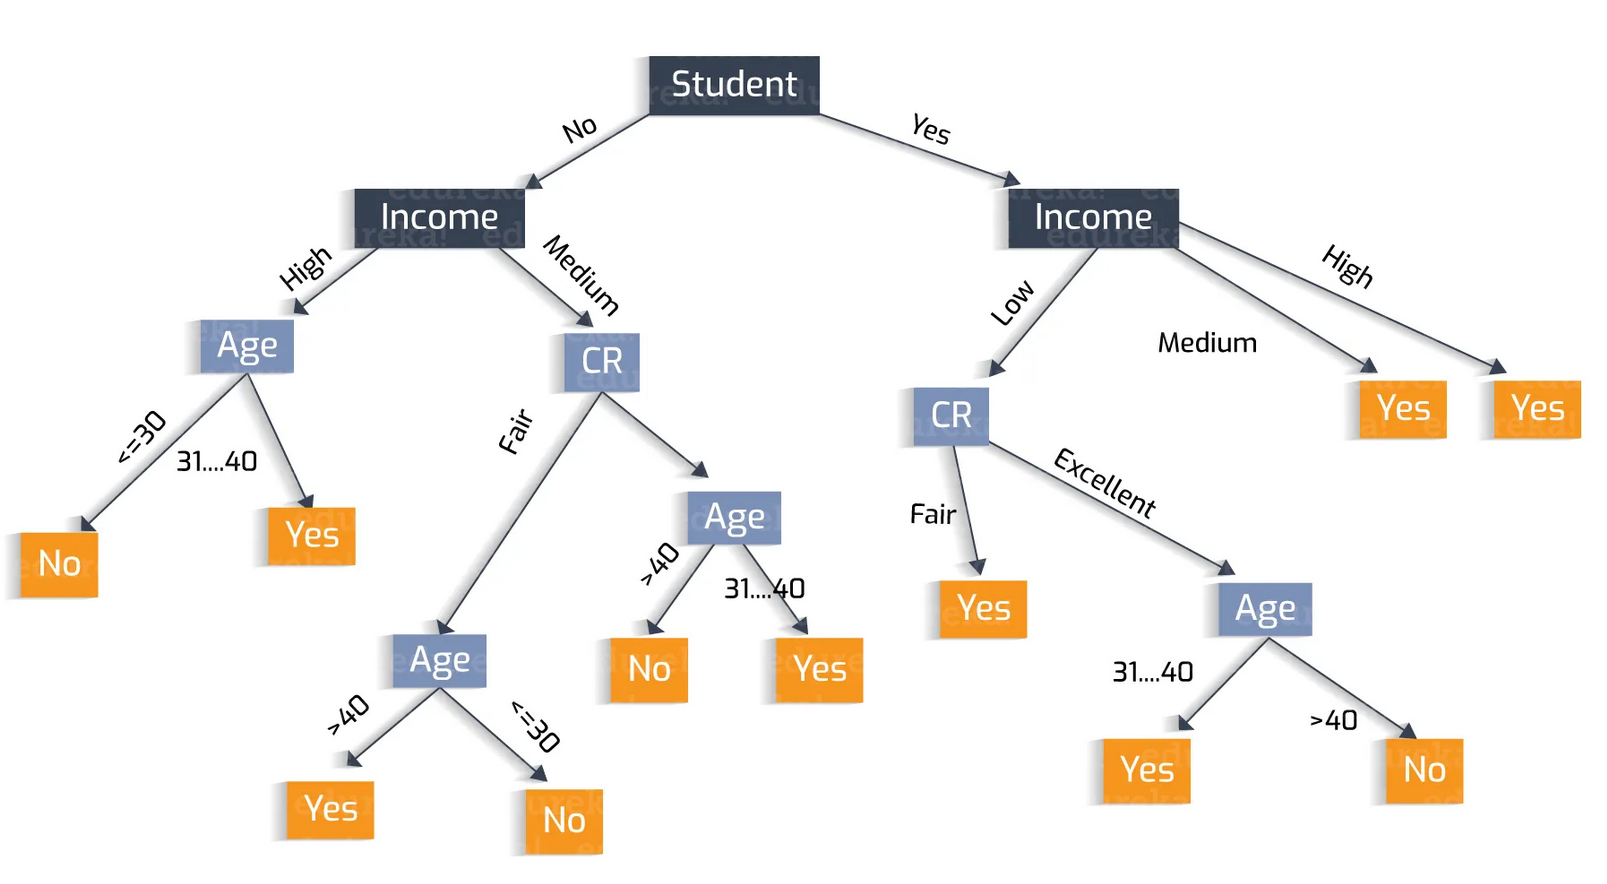
\includegraphics[width=0.7\linewidth]{immagini/decisionTree.png}
		\caption{Esempio di albero di decisione}
		\label{fig:DecisionTree}
	\end{figure}
	La costruzione di un albero di decisione parte individuando la variabile di predizione più importante che viene utilizzata per la suddivisione del primo nodo interno. Questo processo viene ripetuto per ogni sotto-albero fino al raggiungimento di una condizione di stop:
	\begin{itemize}
		\item tutti i campioni di un nodo appartengono alla stessa classe,
		\item non ci sono più attributi per un ulteriore partizionamento,
		\item non rimangono più tuple nelle foglie.
	\end{itemize}
	La partizione risultante a seguito di una divisione usando l'attributo selezionato dovrebbe essere pura, ovvero quando tutte le tuple di una data partizione appartengono alla stessa classe. 
	Per scegliere l'attributo su cui effettuare uno \textit{split} vengono comunemente utilizzati due criteri: la Gini impurity e l'entropia.
	
	La \textit{Gini impurity} misura la probabilità che un elemento scelto a caso appartenente a una data classe sia etichettato in modo errato. Un valore basso indica una maggiore purezza delle classi risultanti dallo split.
	L'entropia è una misura dell'incertezza associata alle classi. Anche in questo caso, un valore basso indica una maggiore purezza delle classi risultanti dallo split.
	Il criterio di scelta può essere utilizzato per valutare tutti gli attributi disponibili e scegliere quello che produce lo \textit{split} con il valore più basso.
	In generale si usano questi criteri per evitare \textit{overfitting} e aiutare a generalizzare meglio il modello su dati sconosciuti.
	Tutte queste tecniche sono euristiche e riescono a trovare un albero efficiente che però non corrisponde all'ottimo, la ricerca dell'albero ottimale è computazionalmente difficile perché il numero di possibili alberi cresce molto rapidamente con il numero di attributi. Prendiamo, per esempio, un insieme di dati con un numero di attributi pari a $n$ che ha solo due valori possibili per ogni attributo, ci sono così $2^n$ possibili alberi di decisione. Se invece ci fossero stati $m$ valori possibili per ogni attributo, allora ci sarebbero stati $m^n$ possibili alberi di decisione.
	
	La ricerca dell'albero ottimo necessita quindi l'esplorazione di tutte queste possibilità e successivamente la valutazione di quale sia l'albero che ha il minor errore sui dati di addestramento. Per questo motivo vengono usati algoritmi \textit{greedy} che creano l'albero prendendo decisioni localmente ottime usando la \textit{Giny Impurity} o l'entropia.


	\subsubsection{Random Forest}
	\label{RandomForest}
	Random forest è una tecnica di apprendimento automatico che si basa sull'utilizzo di molti alberi di decisione per creare un modello più robusto con una precisione migliore rispetto a usare un singolo albero. Esistono diversi motivi per cui si preferisce usare random foresti piuttosto che un singolo albero di decisione:
	\begin{itemize}
		\item miglioramento della precisione: usando più alberi di decisione di solito la precisione finale del modello aumenta,
		\item riduzione dell'\textit{overfitting}: i singoli alberi di decisione possono soffrire di \textit{overfitting}, fenomeno in cui il modello si adatta troppo bene ai dati usati nell'addestramento e non riesce a generalizzare bene sui dati non usati nell'addestramento. Random Forest utilizza una serie di alberi di decisione e prende la decisione finale come voto di maggioranza, riducendo così l'effetto dell'\textit{overfitting},
		\item rilevamento di feature importanti: permette di individuare quali sono le feature più importanti per classificare i dati,
		\item scalabiltà: scala molto bene con dataset grandi.
	\end{itemize}
	
	\subsection{Apprendimento non supervisionato}
	Nell'apprendimento non supervisionato si ha un insieme di $N$ osservazioni $x_1, x_2,...,x_N$ di un vettore avente $p$ dimensioni ma, al contrario dell'apprendimento supervisionato, l'insieme di dati non ha un'etichetta, i dati sono quindi non annotati.
	Nel contesto dell'apprendimento supervisionato ci sono diverse metriche che mi indicano quanto il modello è stato in grado di ``imparare''. Nel contesto dell'apprendimento non supervisionato non esiste una vera e propria misura diretta del successo di un algoritmo. È molto difficile accertare la validità delle inferenze tratte dall'output e dipendono dal tipo di problema e dall'algoritmo utilizzato. A questo scopo si deve ricorrere a euristiche per valutare la qualità dei risultati ottenuti. È importante notare che in genere vengono utilizzate più metriche per valutare l'apprendimento non supervisionato in modo da avere una valutazione completa. 
	
	\subsection{Apprendimento semi-supervisionato}
	L'apprendimento semi-supervisionato è un tipo di apprendimento automatico in cui dei dati che vengono passati all'algoritmo solamente una piccola parte è etichettata. L'obiettivo dell'algoritmo è quello di usare i dati etichettati per riuscire a fornire una etichetta automaticamente anche ai dati che ne sono privi. Esistono diverse tecniche per fare ciò, come ad esempio le tecniche di propagazione delle etichette \cite{LearningfromLabeledandUnlabeledDatawithLabelPropagation}, le tecniche di co-training \cite{10.1145/279943.279962}, le tecniche di self-training \cite{inproceedings}.
	
	
	\subsection{Apprendimento per rinforzo}
	L'apprendimento per rinforzo è un tipo di apprendimento automatico in cui troviamo un agente che interagisce con uno specifico ambiente in modo da ottenere una ricompensa. L'obiettivo è quello di imparare a prendere decisioni e azioni massimizzando la ricompensa. L'apprendimento per rinforzo si compone di diverse fasi:
	\begin{itemize}
		\item l'agente inizialmente agisce in maniera casuale non avendo nessuna conoscenza dell'ambiente, 
		\item interagendo con l'ambiente l'agente inizia a prendere decisioni e ottenere così le ricompense,
		\item ottenendo le ricompense l'agente ``capisce'' come deve agire e adatta la sua \textit{policy}, l'obiettivo è sempre massimizzare la ricompensa.
	\end{itemize}
	L'agente utilizza una funzione di valore per valutare le azioni e aiutarlo a scegliere quale azione prendere in un determinato contesto. Esistono diverse funzioni che vengono comunemente usate: funzione di valore Q, funzione di valore V e  funzione di valore di \textit{policy} \cite{busoniu2010reinforcement}.
	
	\section{Apprendimento automatico in bioinformatica}
	L'apprendimento automatico viene utilizzato in tantissimi ambiti di ricerca \cite{Sarker2021}: analisi predittiva e processo decisionale intelligente, sicurezza informatica, \textit{Internet of things} e città smart, previsione del traffico, trasporto pubblico, \textit{healthcare}, pandemia dovuta al COVID-19, NLP, ecc.
	Questa tecnologia trova spazio anche all'interno della bioinformatica, ovvero l'applicazione di tecniche di calcolo per acquisire e interpretare i dati biologici. È un campo interdisciplinare tra informatica, matematica, statistica, biologia e genetica. 	
	La crescita esponenziale di dati biologici disponibili ha sollevato due problemi: un modo efficiente di immagazzinare e gestire dati di questo tipo e riuscire a sfruttarli riuscendo a estrarre informazioni utili. I domini in cui vengono utilizzate tecniche di machine learning sono molte: in Figura \ref{fig:utilizzimachinelearningbioinfo} vengono mostrate le principali aree nel quale si utilizzano metodi computazionali. All'interno troviamo sei diversi domini: genomica, proteomica, microarray, biologia dei sistemi, evoluzione e text mining. Inoltre troviamo una categoria denominata ``other application'' nel quale troviamo i restanti problemi. 
	
	\begin{figure}[h]
		\centering
		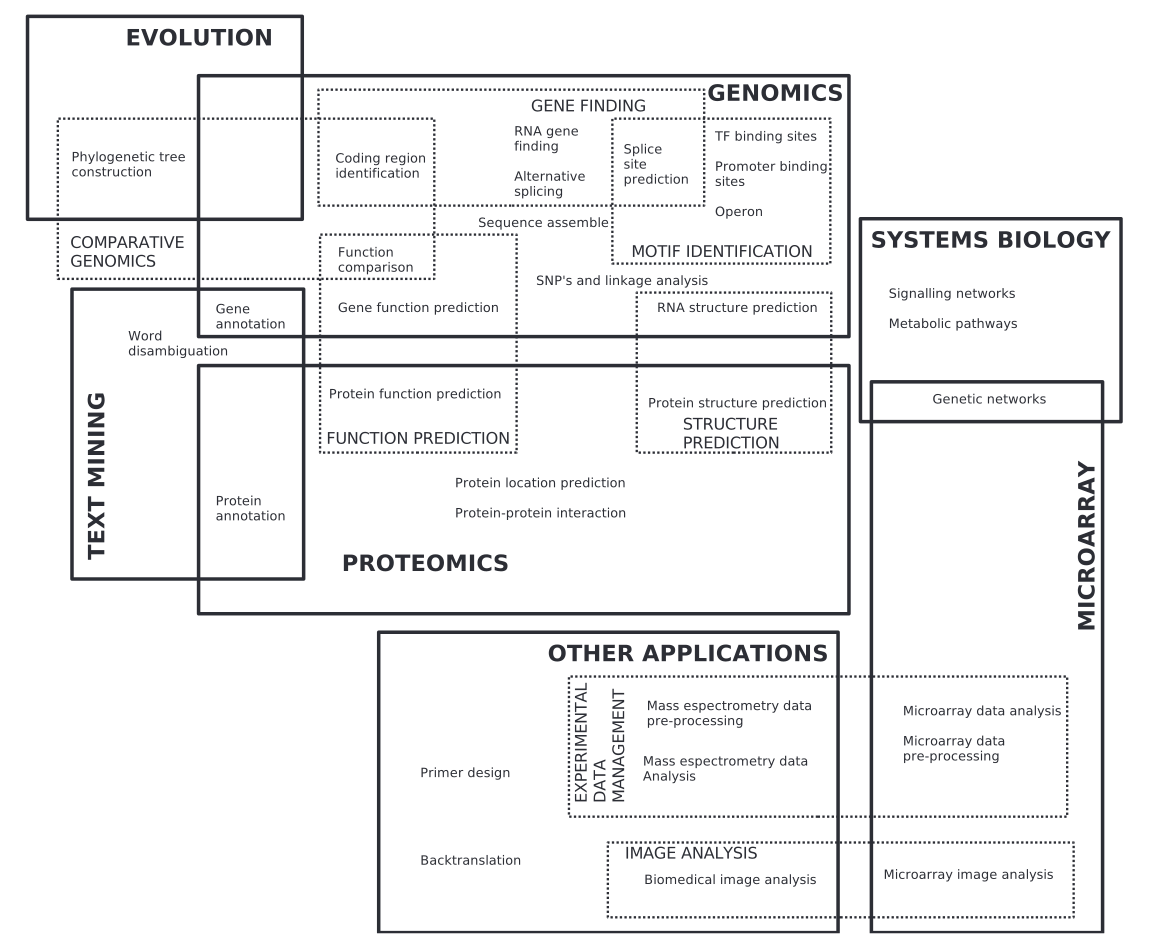
\includegraphics[width=0.8\linewidth]{immagini/utilizziMachineLearningBioinfo}
		\caption[]{Classificazione dei campi in cui vengono applicati metodi di apprendimento automatico in bioinformatica}
		\label{fig:utilizzimachinelearningbioinfo}
	\end{figure}

	La genomica è una delle aree più importanti in bioinformatica. Il numero di sequenze nucleotidiche e proteiche disponibili è in continuo aumento come visibile in figura \ref{fig:growthofgenbank}. GenBank è una banca dati a libero accesso e senza restrizione, istituita nel 1982, che riporta tutte le sequenze di nucleotidi e le relative proteine ottenute dopo la loro traduzione. GenBank riceve le proprie informazioni dai risultati ottenuti su oltre 300.000 distinti organismi da laboratori sparsi in tutto il mondo, rappresentando il più importante punto di riferimento nel suo campo di ricerca. A febbraio 2020, conteneva oltre 216 milioni di loci \footnote{In genetica, il termine locus genico (o più semplicemente locus, plurale loci) designa la posizione, stabile, di un gene o di un marcatore genico all'interno di un cromosoma} e oltre 399 miliardi di basi da più di 216 milioni di sequenze riportate.

	\begin{figure}[h]
		\centering
		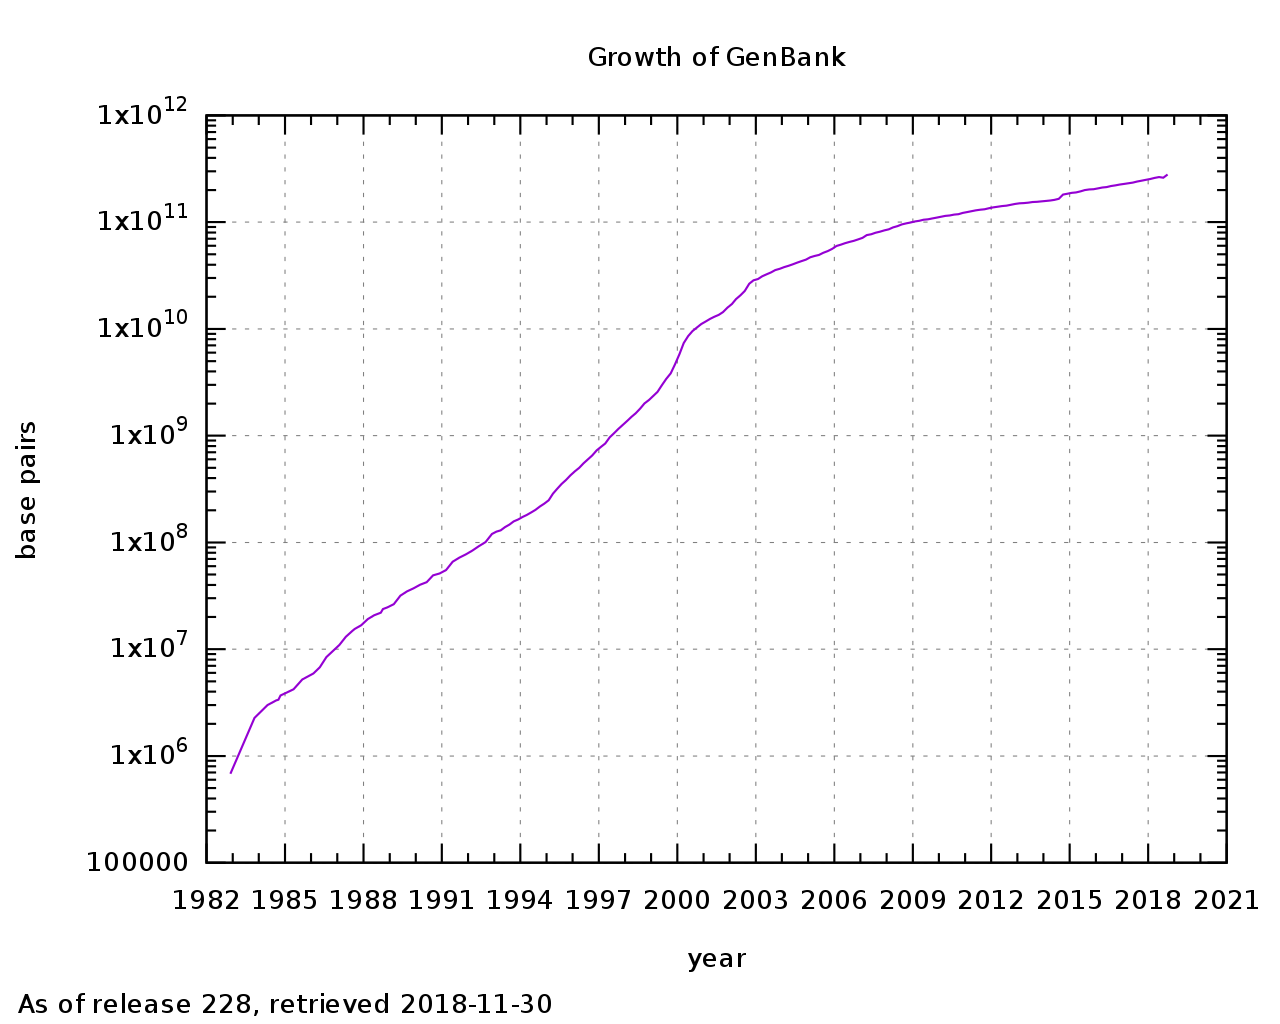
\includegraphics[width=0.6\linewidth]{immagini/Growth_of_Genbank.svg}
		\caption{Crescita di GenBank}
		\label{fig:growthofgenbank}
	\end{figure}
	Tutti questi dati hanno bisogno di essere processati in modo da ottenere informazioni utili. Come prima cosa  è possibile estrarre struttura e posizione dei geni dalle sequenze del genoma \cite{Mathe2002-us}, inoltre è anche possibile identificare gli elementi regolari \cite{Aerts2004-jh}. Esistono inoltre approcci per estrarre caratteristiche comuni tra gli RNA noti per la previsione di nuovi geni RNA nelle regioni non annotate dai genomi procariotici e arcaici \cite{Carter2001-oo}.
	
	Nella proteomica i metodi computazionali vengono usati per la previsione della struttura delle proteine. Le proteine hanno una struttura molto complessa composta da migliaia di atomi e legami, di conseguenza il numero di possibili strutture è estremamente elevato. La previsione della struttura risulta quindi un problema combinatorio molto complesso e richiede una buona ottimizzazione.
	
	Attraverso l'applicazione dei metodi computazionali è possibile anche gestire dati sperimentali complessi, il campo più noto dove troviamo applicazioni di questo tipo sono i \textit{microarray} \footnote{Si tratta di sottili supporti di materiale plastico o vetro su cui si trovano molte migliaia di pozzetti, ciascuno contenente pochi picogrammi ($1$ pg = $10$-$12$g) di una diversa sonda di DNA a singola elica.} nel quale si cerca di identificare i pattern di espressione, cercare una classificazione e creare reti genetiche.
	  
	
	Passiamo ora a vedere alcuni esempi pratici di applicazione di tecniche di apprendimento automatico in campo bioinformatico e medico.
	
	\subsection{Apprendimento automatico per la previsione di varianti non codificanti associate a malattie}
	All'interno di tutte le variazioni genetiche quelle riguardanti le malattie rappresentano una piccolissima minoranza rispetto all'insieme più ampio di variazioni genomiche non deleterie. Questo squilibrio porta a un sbilanciamento tra gli insiemi, sopratutto nelle regioni regolatore non codificanti del genoma umano. 
	Quello che si vorrebbe fare è usare tecniche di apprendimento automatico per individuare varianti non codificanti associate alle malattie ma la scarsità di osservazioni inficia sulla loro efficacia. Lo stato dell'arte dei metodi basati sull'apprendimento automatico non adottano tecniche specifiche che tengono conto dello sbilanciamento dei dati e questo porta inevitabilmente a una riduzione della sensibilità e della precisione.
	
	In questo contesto gli algoritmi di apprendimento classici come \textit{support vector machine} \cite{Cortes1995} o \textit{artificial neural networks} \cite{bishop1995neural} non riescono a generalizzare in maniera sufficiente poiché di solito prevedono la classe di minoranza con una precisione e sensibilità molto bassa.
	Nel campo della previsione di varianti genetiche associate a tratti o malattie, ciò si riduce a prevedere erroneamente la maggior parte delle varianti associate alla malattia come non associate alla malattia stessa, limitando così in modo significativo l'utilità dei metodi di apprendimento supervisionato per la previsione di nuove varianti non codificanti associate alla malattia.
	
	Per affrontare questo problema è stato sviluppato \textit{hyper}SMURF \cite{Schubach2017} sigla che sta a indicare: \textit{hyper-ensemble of SMOTE Undersampled Random Forest}. Questo metodo adotta strategie di apprendimento che tengono conto dello sbilanciamento, ovvero tecniche di ricampionamento e su un approccio \textit{hyper-ensemble}: simultaneamente la classe di minoranza viene sovracampionata e la classe di maggioranza viene sottocampionata in modo da generare dati di addestramento bilanciati, ciascuno dei quali verrà poi usato per addestrare un insieme di random forest \ref{RandomForest}. La sua struttura è visibile in Figura \ref{fig:hypersmurf}.
	\begin{figure}[h!]
		\centering
		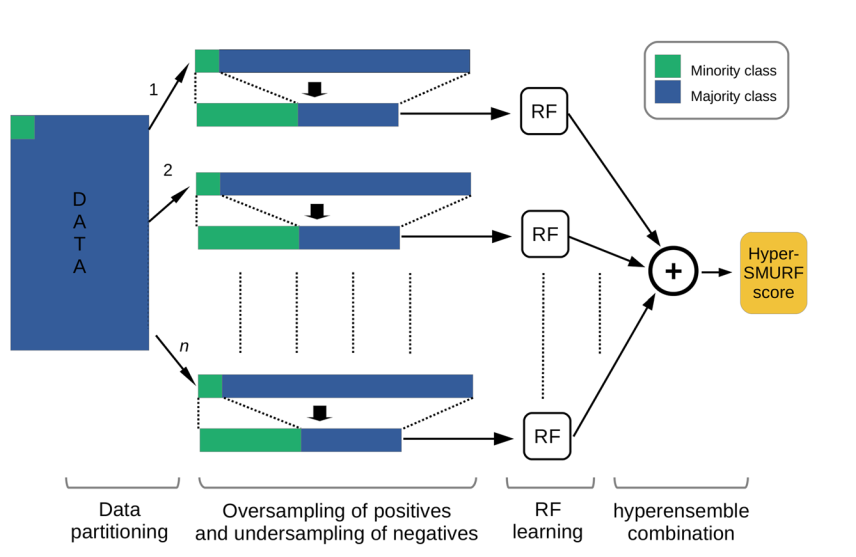
\includegraphics[width=0.7\linewidth]{immagini/hyperSMURF}
		\caption{Schema di \textit{hyper}SMURF. Esso divide la classe maggioritaria (rettangoli blu) in $n$ partizioni e per ognuna di esse vengono usate tecniche di sovracampionamento in modo da generare esempi aggiuntivi dalla classe minoritaria (rettangoli verdi). Contemporaneamente un numero simile di esempi viene sottocampionato dalla classe maggioritaria. Successivamente \textit{hyper}SMURF addestra in parallelo $n$ random forest usando i dati bilanciati e infine combina le predizioni degli $n$ insimi secondo un approccio \textit{hyper-ensemble}}.
		\label{fig:hypersmurf}
	\end{figure}

	Successivamente le predizioni dei modelli addestrati sono combinati attraverso un approccio chiamato \textit{hyper-ensemble}, insieme di insiemi, per ottenere una predizione complessiva ``concordata''. Addestrando $n$ \textit{random forest}, una per ogni insieme di dati, e combinando le loro previsioni facendo la media delle probabilità si ottiene un \textit{hyper-ensemble} poiché ogni dato passato è a sua volta un insieme di alberi decisionali.
	
	Il vantaggio risiede nel fatto di avere molta diversità nei dati di addestramento, inoltre il bilanciamento tra esempi positivi e negativi evitano che si abbia una polarizzazione verso la classe maggioritaria. Tutto ciò rende il modello più capace di generalizzare, mentre l'approccio di \textit{hyper-ensemble} fornisce apprendimento più accurato e previsioni più robuste.
	Per testare il modello viene utilizzato una 10-\textit{cross-validation} per assicurarsi che le varianti della stessa malattia non si presentino insieme nel \textit{training set}, o insieme di addestramento, e in quello di test, falsando così i risultati. La misura vera e propria è affidata all'AUPRC, ovvero \textit{Area Under the Precision and Recall}, all'AUROC, \textit{Area Under the Receiver Operating Characteristic} e usando la precisione, il richiamo e il punteggio F in funzione della soglia di punteggio.
	
	\begin{figure}[h]
		\centering
		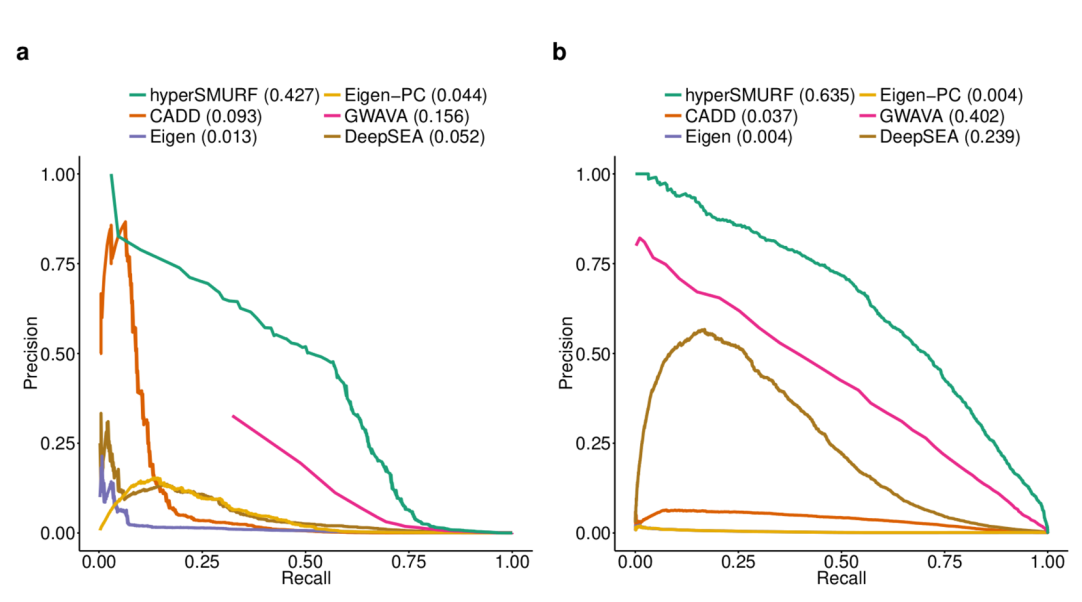
\includegraphics[width=0.7\linewidth]{immagini/ResultHyperSMURF}
		\caption{Confronto della curva \textit{precision/recall} tra i vari modelli usando due tipi diversi di dati: a) \textit{Mandelian regulatory mutations}, b) \textit{GWAS regulatory hits}. Il numero tra parentesi rappresenta il valore di AUPRC.}
		\label{fig:resulthypersmurf}
	\end{figure}

	I risultati sono visibili in figura \ref{fig:resulthypersmurf} dove è possibile vedere un confronto tra i vari metodi usando la curva \textit{prevision-recall}. Si nota chiaramente come \textit{hyper}SMURF raggiunge migliori risultati rispetto ai metodi classici.
	
	
	\subsection{Apprendimento automatico per la previsione del rischio di COVID-19}
	Negli ultimi anni una grave sindrome respiratoria (SARS-Cov-2) ha colpito il mondo provocando una pandemia mondiale causando $663$ milioni di casi accertati e quasi $7$ milioni di morti accertati\footnote{https://ourworldindata.org/covid-deaths}.

	\begin{figure}
		\centering
		\begin{subfigure}[b]{0.4\textwidth}
			\centering
			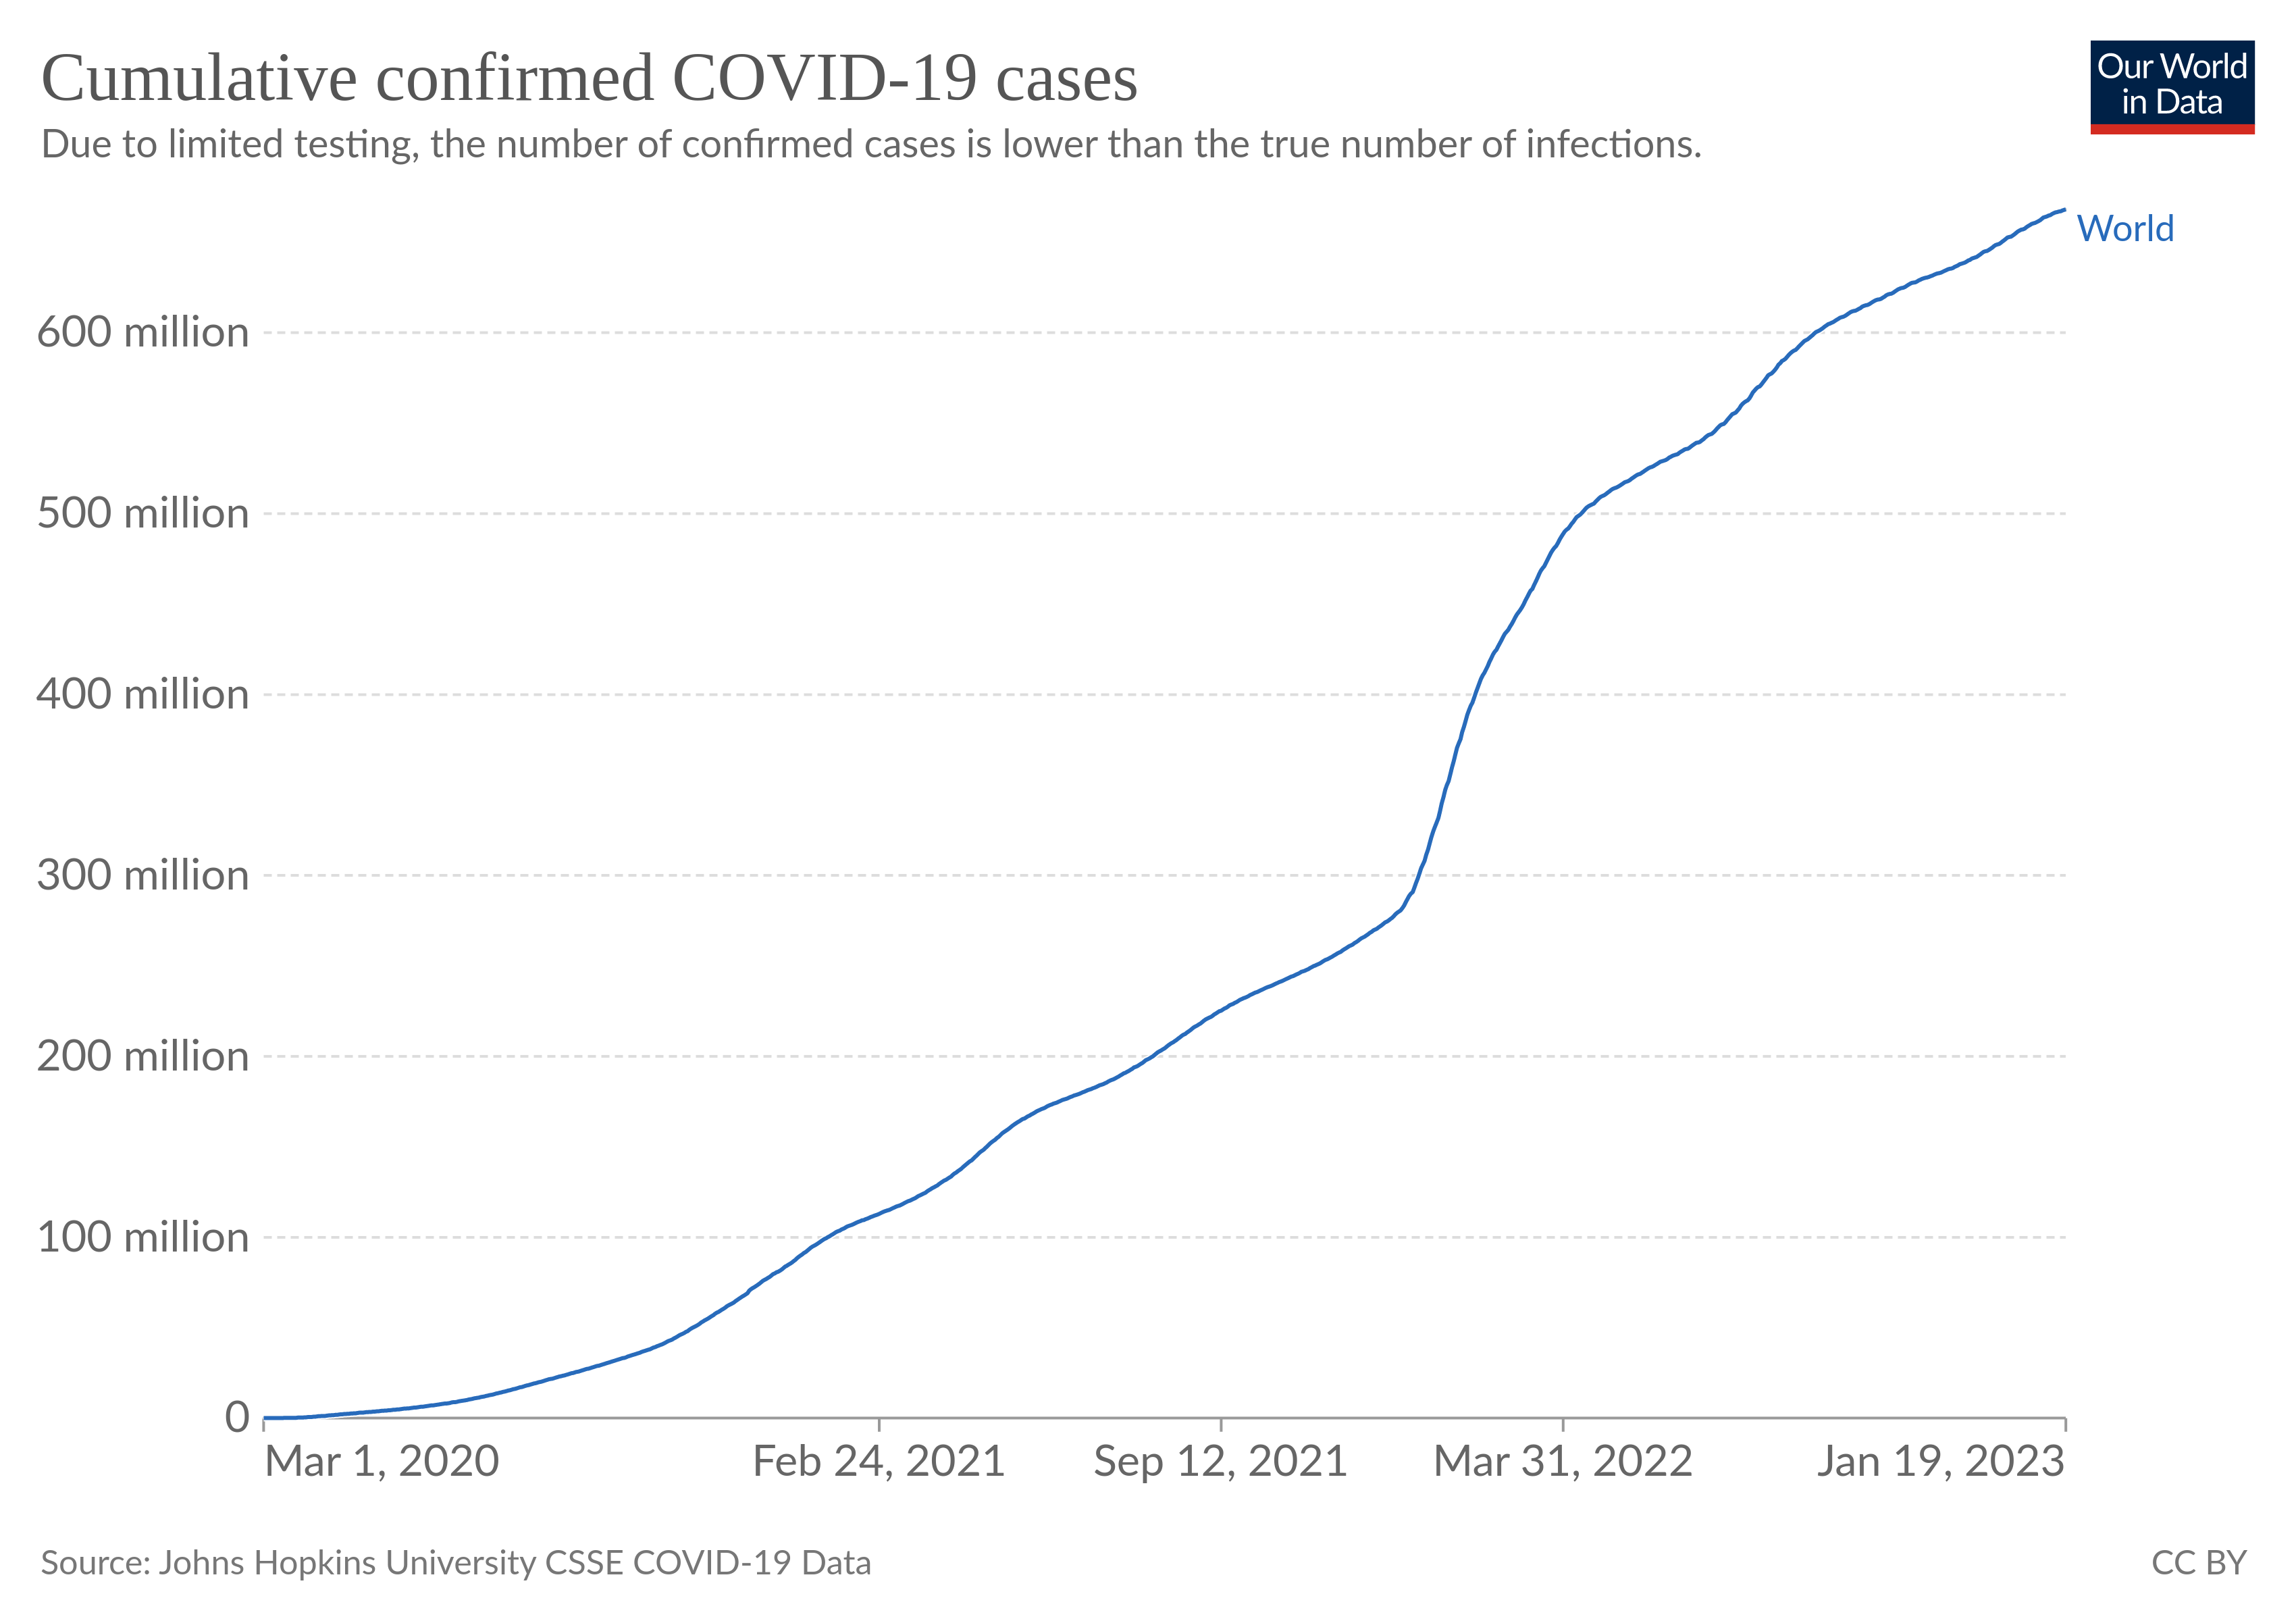
\includegraphics[width=0.9\linewidth]{immagini/coronavirus-data-explorer_cases}
			\caption{}
			\label{fig:coronavirus-data-explorercases}
		\end{subfigure}
		\begin{subfigure}[b]{0.4\textwidth}
			\centering
			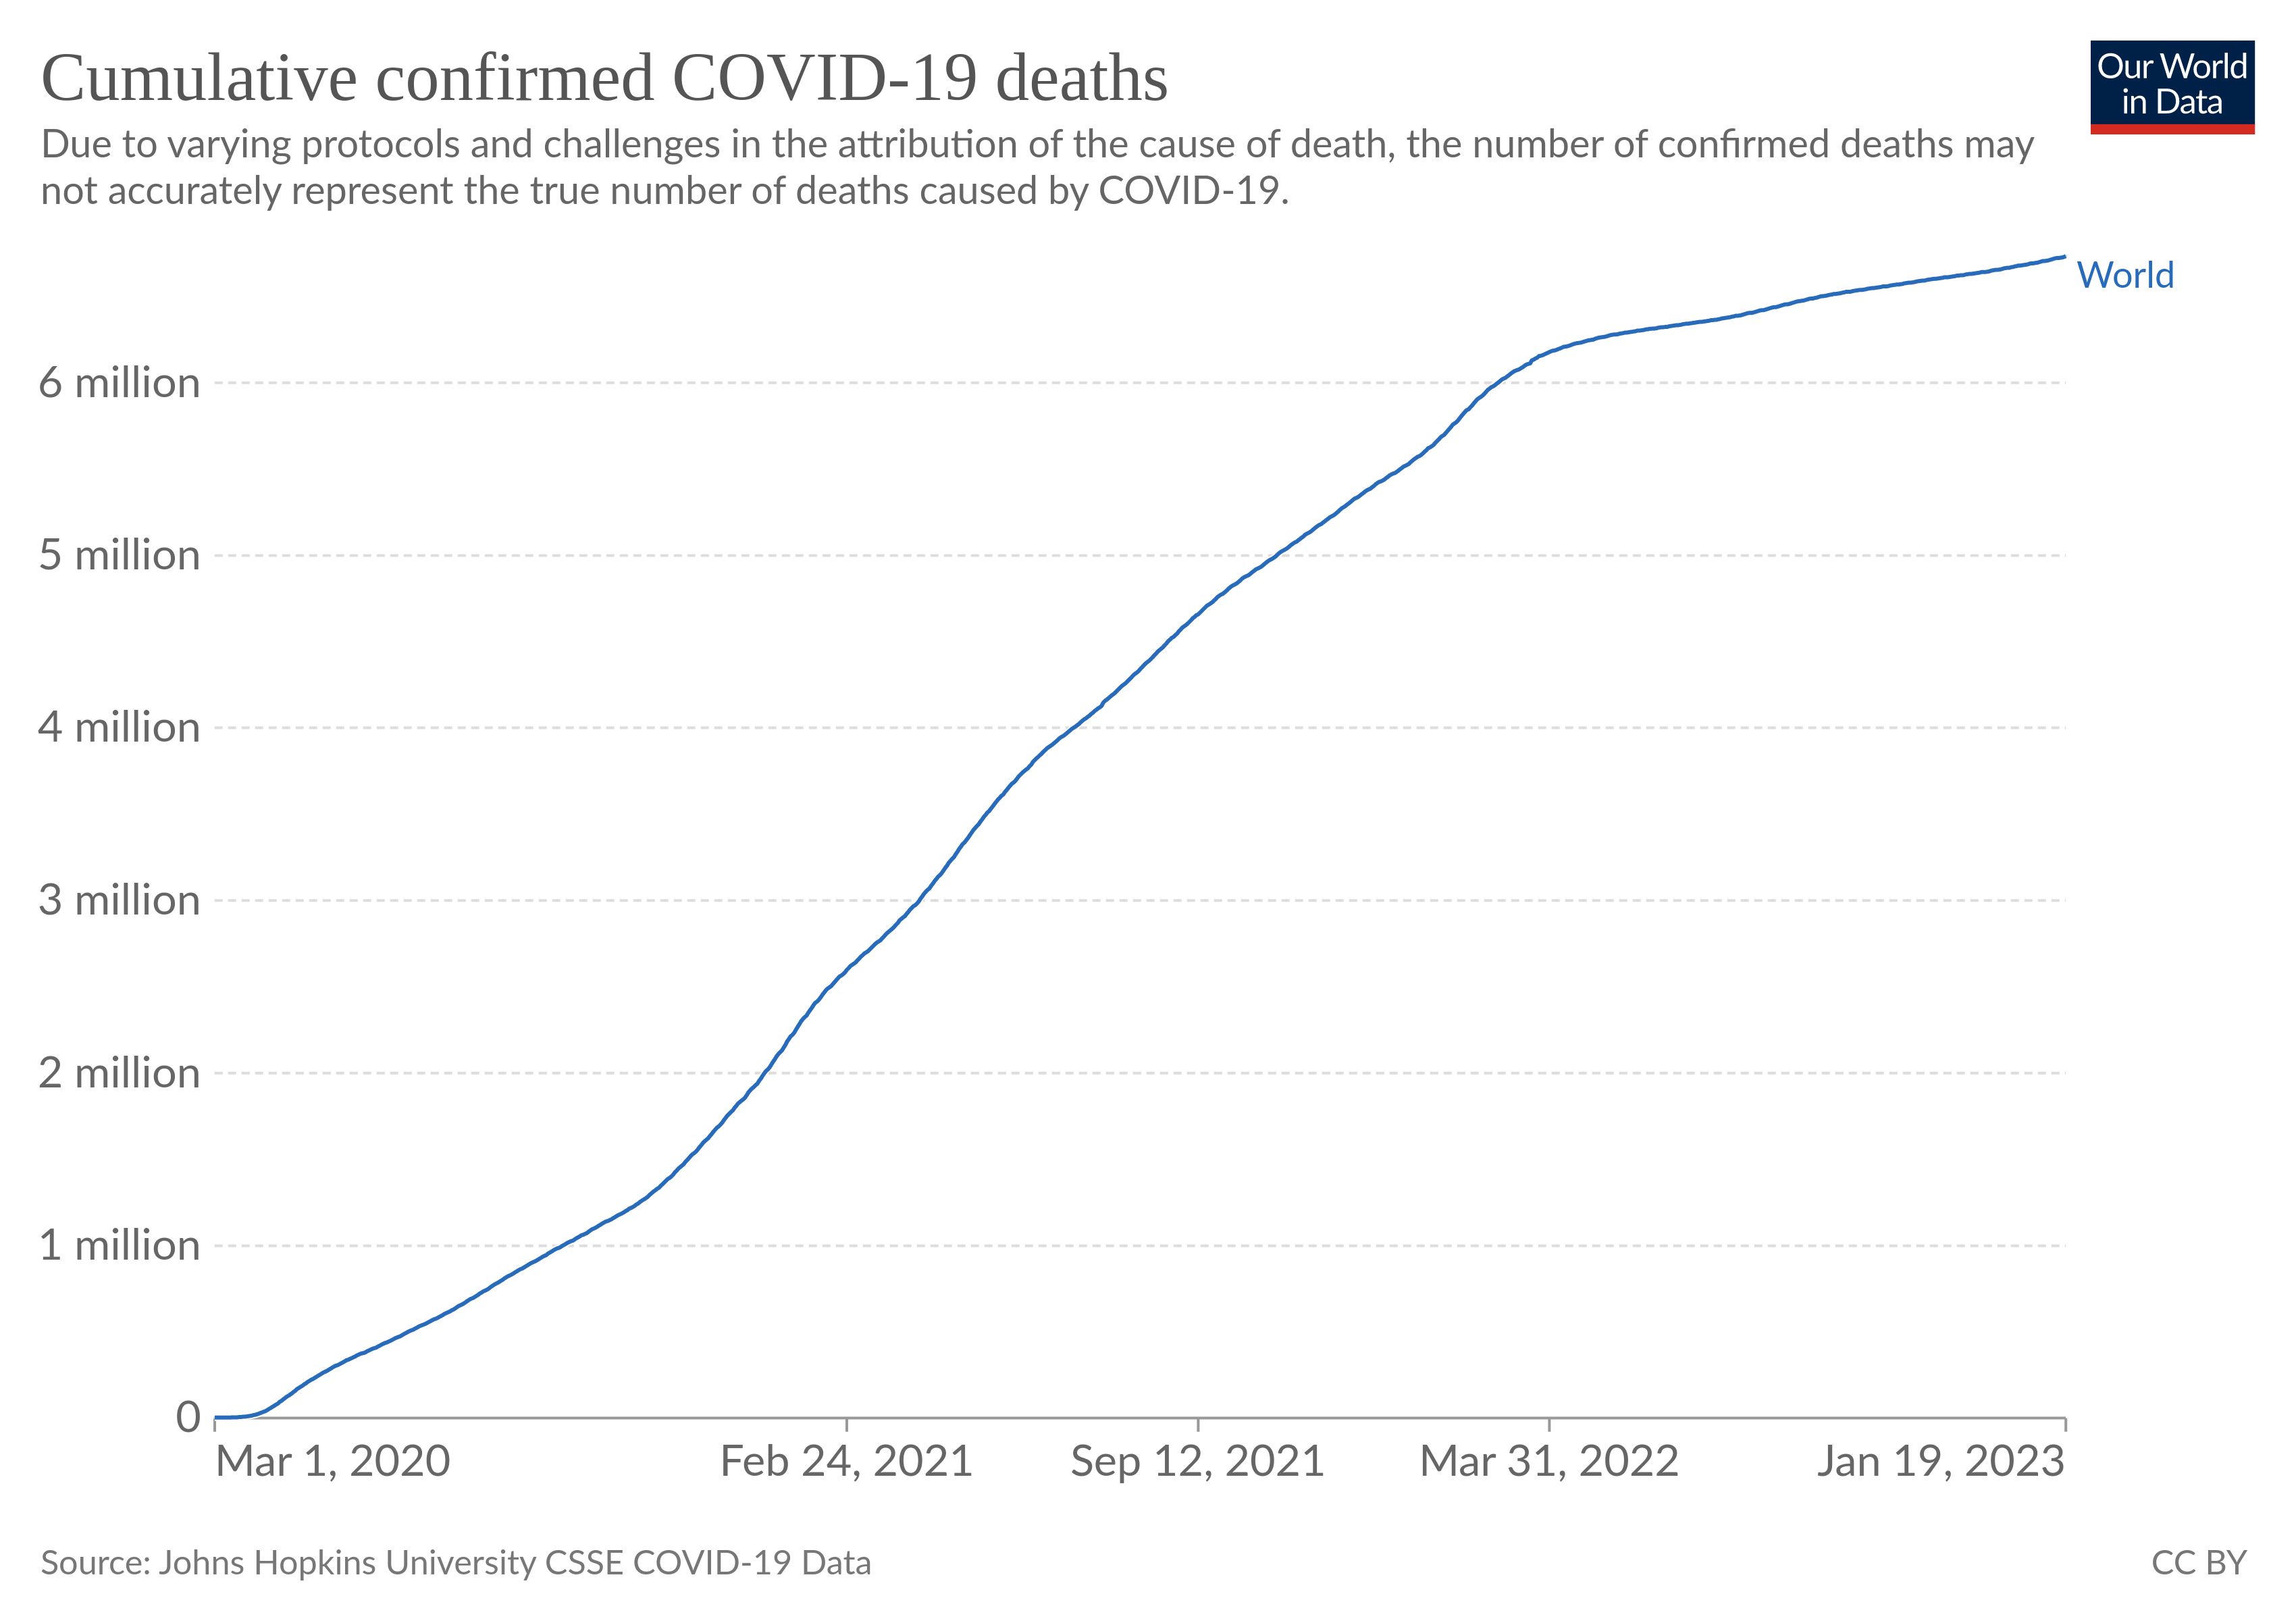
\includegraphics[width=0.9\linewidth]{immagini/coronavirus-data-explorer_death}
			\caption{}
			\label{fig:coronavirus-data-explorerdeath}
		\end{subfigure}
	\caption{Grafico che mostra a) casi totali nel mondo da quando è scoppiata la pandemia a oggi; b) morti totale nel mondo da quando è scoppiata la pandemia a oggi.}
	\label{fig:COVID_deaths_and_cases}
	\end{figure}

	Da quando il virus ha iniziato a diffondersi tra la popolazione ospedali e pronto soccorsi sono stati invasi da pazienti per i quali era necessario sapere se avessero contratto la malattia o meno ma sopratutto la gravità. Il virus è in grado di causare anomalie nelle radiografie del torace (CXR) ma a causa della sua bassa sensibilità sono necessari ulteriori considerazioni e criteri per riuscire a prevedere il rischio di aver contratto il virus con conseguente gravità.
	L'obiettivo è quello di riuscire a creare un sistema che riesca a estrarre le variabili ragiologiche, cliniche e di laboratorio più rilevanti che siano in grado di migliorare la previsione del rischio del paziente. Si vogliono inoltre ottenere criteri utilizzabili dai medici nel momento in cui devono decidere il rischio del paziente, intesa come gravità della malattia. In \cite{Casiraghi2020-zt} viene illustrato un modello di previsione del rischio per il paziente. Il modello è in grado di selezionare le più importanti variabili cliniche e di laboratorio tenendo anche conto di punteggi radiologici che derivano dalla valutazione del CXR \footnote{\textit{Chest-X-Ray}} da parte dei radiologi e due punteggi di "coinvolgimento polmonare" calcolati usando alcune delle \textit{deep neural network} più performanti per la diagnosi del rischio da COVID-19.
	Successivamente viene eseguita una fase di imputazione dei dati mancanti causata dall'integrazione di più fonti di dati. Le tecniche usate sono state la \textit{Multiple Imputations by Chained Equations} (MICE \cite{JSSv045i03}), sia utilizzando la corrispondenza media predittiva (\textit{micePPM}), sia classificatori random forest (\textit{miceRF})  come modello di imputazione di bas, e \textit{missForest} \cite{10.1093/bioinformatics/btr597}.
	In seguito viene costruito un algoritmo robusto che combina Boruta \cite{JSSv036i11} \cite{Kursa2010} con metodi di selezione delle caratteristiche, o (\textit{features}), basati sulle permutazioni e incorporati nelle Random Forest \cite{Altmann2010-sw} \cite{Strobl2007}.
	
	Le \textit{feature} selezionate sono usate come input per random forest (RF) \ref{RandomForest} e per alberi associativi derivati (AT) \cite{e1bb70540db14ceeacddd4383fca9bff}. A differenza delle RF che producono un gran numero di regole di difficile comprensione, le AT sono costruite partendo dalle RF ma producendo un numero regole più semplice che può essere facilmente valutato e interpretato dai medici.
	I risultati ottenuti dai due algoritmi sono comparati a quelli ottenuti dai modelli generalizzati (GLM \cite{10.2307/2344614}) eliminando così l'ipotesi di normalità. 
	
	\begin{figure}[h]
		\centering
		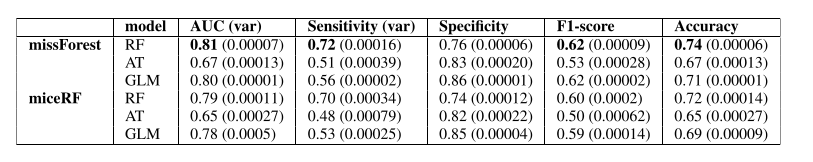
\includegraphics[width=0.8\linewidth]{immagini/resultCovidModel}
		\caption{Tabella con le misure di performance calcolate usando i vari algoritmi}
		\label{fig:resultcovidmodel}
	\end{figure}
	
	
	\chapter{Dataset}
	Un insieme di dati, chiamato \textit{dataset} in inglese, è una raccolta di dati in cui ogni riga rappresenta un'osservazione, o istanza, e ogni colonna costituisce un attributo, o caratteristica, dell'istanza.
	
	L'apprendimento automatico ha bisogno di dati per poter addestrare i modelli. L'obiettivo è riuscire a creare modelli che siano in grado di generalizzare e prevedere correttamente al passaggio di nuovi dati. I dati possono influire significativamente sulle prestazioni nelle predizioni, pertanto è importante utilizzare un insieme di dati ben equilibrato, rappresentativo e qualitativo.

	Nel mio lavoro ho usato apprendimento supervisionato quindi l'insieme di dati aveva anche un'etichetta. L'obiettivo è addestrare il modello in modo che riesca a estrapolare la relazione che sussiste tra i dati, $X$, e l'etichetta, $y$, per far si che, al passaggio di nuove istanze, esso mi restituisca l'etichetta predetta sulla base dei dati passati.
	
	\section{Dati Multi-Omici}
	I dati multi-omici sono un insieme dei dati che contengono le variazioni molecolari su più livelli quali: genomica, epigenomica, trascrittomica, proteomica, metaboloma e microbiotica. La disponibilità di questo tipo di dati ha completamente rivoluzionato il campo della medicina e della biologia.
	
	La genomica è il campo che si occupa dell'identificazione dei geni e delle varianti geniche associate a una malattia o in risposta a determinati medicinali. 
	
	Il termine epigenomica si riferisce all'identificazione di modificatori di DNA o delle proteine associate al DNA. Le modifiche epigenetiche del genoma possono anche agire come marcatori per sindromi metaboliche, malattie cardiovascolari e disturbi fisiologici. Queste modifiche possono essere specifiche per cellula e tessuto, è quindi fondamentale identificare le modifiche epigenetiche durante gli stati nativi della malattia.
	
	La trascrittomica esamina i livelli di RNA in tutto il genoma, sia in modo quantitativo che qualitativo, includendo quali trascrittori sono presenti e i livelli della loro espressione. Sebbene solo il $2\%$ del DNA venga tradotto in proteine, quasi l'$80\%$ del genoma viene trascritto, tale processo include l'RNA codificante, RNA corto, microRNA, piwi RNA e piccoli RNA nucleari. Oltre a fungere da intermediario tra DNA e proteine, l'RNA ha anche funzioni strutturali e regolatorie. E' stato dimostrato che essi hanno un ruolo nell'infarto miocardico, nella differenziazione adiposa, nel diabete, nella regolazione endocrina, nello sviluppo neuronale e altri \cite{Hasin2017},
	
	Il termine proteomica indica il campo nel quale si cerca di identificare i livelli, le modifiche e le interazione delle proteine a livello del genoma. Queste modifiche sono coinvolte nella manutenzione della struttura e della funzione cellulare. 
	
	Il metaboloma comprende tutti i metaboliti presenti in una cellula, tessuto o organismo, compresi i piccoli molecolari, carboidrati, peptidi, lipidi, nucleotidi e i prodotti catabolici. Rappresenta il prodotto finale della trascrizione genica e consiste sia di molecole di segnalazione che strutturali. La dimensione del metaboloma è molto più piccola rispetto alla dimensione del proteoma e quindi è più facile da studiare.
	
	Infine la microbiomica consiste in tutti i microorganismi di una comunità. I microbi sono ovunque, sono stati trovati sulla pelle umana, sulle superfici mucose e nell'intestino. Il microbiome presente negli esseri umani è molto complesso, per esempio nell'intestino troviamo circa 100 trilioni di batteri.
	La microbiota è stata trovata coinvolta in diabete, obesità, cancro, colite, malattie cardiache e autismo. Pertanto, la caratterizzazione del microbiome o di un organismo è di grande interesse medico.
	
	Grazie alla ricerca ci sono stati progressi in diversi campi omici e si è capito che la risposta a una domanda non è da ricercare in un solo tipo di dato poiché questi dati si influenzano tra di loro, esempio il microbiome influenza l'espressione genica e proteica che a sua volta influenza il metabloma. È quindi necessario studiare i dati nella loro interezza sfruttando i dati multi-omici per comprendere lo stato nativo e alterato di un organismo attraverso l'analisi dei dati provenienti da diverse fonti omiche.
	
	\begin{figure}[h]
		\centering
		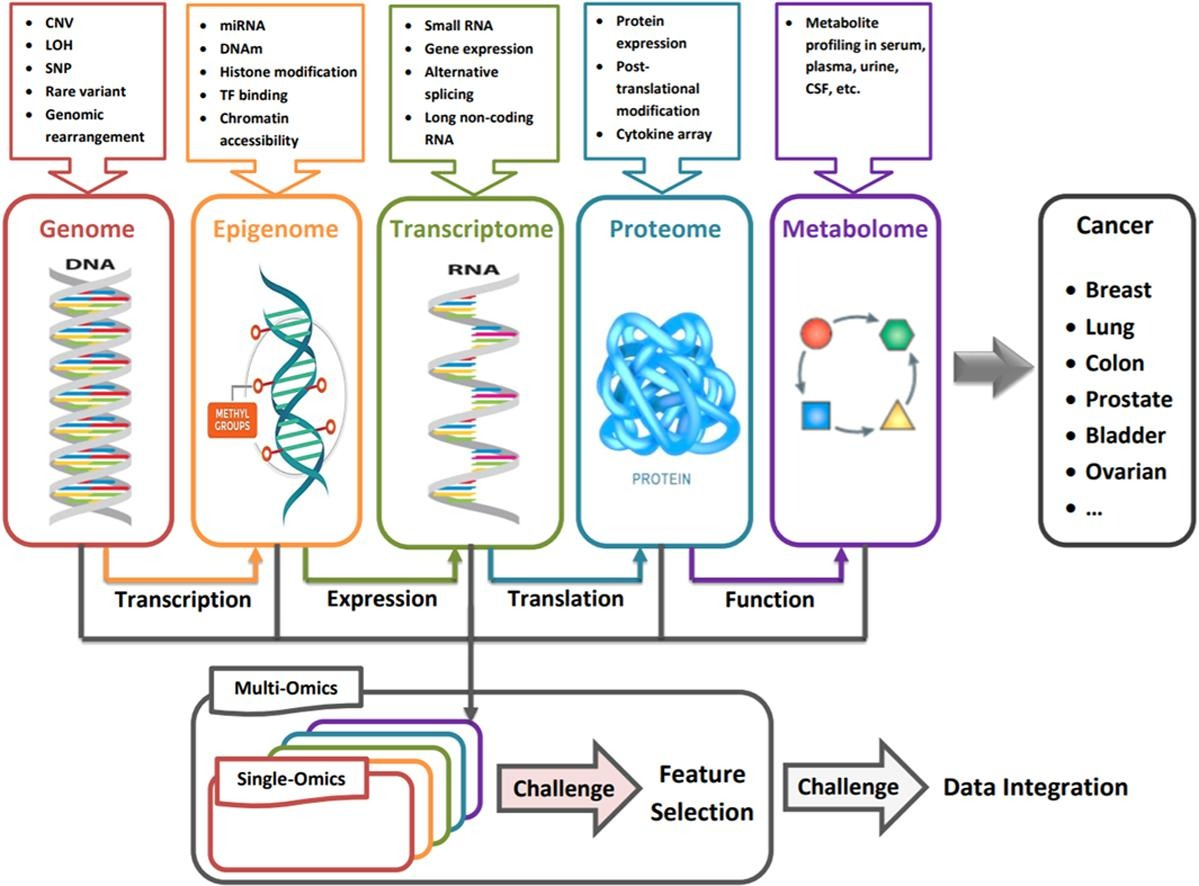
\includegraphics[width=0.7\linewidth]{immagini/multi-omicsData}
		\caption{Diagramma delle relazioni tra i vari tipi di dati omici}
		\label{fig:multi-omics}
	\end{figure}
	
	Esistono diversi database che forniscono dati multi-omici di pazienti, uno di questi è il \textit{The Cancer Genome Atlas}.
	
	\subsection{The Cancer Genome Atlas (TCGA)}
	Il Cancer Genome Atlas è il programma di riferimento per la genomica del cancro, ha favorito la caratterizzazione sistematica di diverse alterazioni genomiche alla base dei tumori umano. Attualmente ha caratterizzato oltre 11000 tumori di 33 tipi di cancro. Si tratta di uno sforzo congiunto tra Nation Cancer Institute e il National Human Genome Research Institute e riunisce ricercatori di diversi discipline e istituzioni\cite{TCGA}.

	I dati utilizzati sono stati presi da TCGA tramite il package curatedTCGAData \footnote{https://bioconductor.org/packages/release/data/experiment/html/curatedTCGAData.html}. Essi sono dati sul carcinoma mammario invasivo (TCGA-BRCA). Questo è un tipo di cancro che si sviluppa all'interno della mammella ed è in grado di diffondersi alle altri parti del corpo attraverso linfonodi o vasi sanguigni. I dati sono stati ottenuti facendo riferimento alla versione del genoma umano hg19, questa versione è stata pubblicata nel 2009 dal progetto internazionale del genoma umano (IGHP) \footnote{https://www.genome.gov/human-genome-project} e contiene informazioni sulla sequenza del DNA umano, sequenze dei geni, i siti di regolazione genica e le regioni non codificanti del DNA. 
	Nello specifico, le tipologie di dati utilizzate sono le seguenti:
	
	\subsubsection{Proteine}
	Rappresentano i livelli di espressione delle proteine. Le proteine sono le macromolecole che svolgono essenzialmente ogni compito all'interno della cellula. Tra queste, i più importanti sono:
	\begin{itemize}
		\item strutturali: alcune proteine formano la struttura delle membrane cellulari e altre sostengono la forma della cellula,
		\item catalitiche: molte proteine sono enzimi, che catalizzano reazioni chimiche all'interno della cellula,
		\item regolatorie: alcune proteine regolano l'espressione genica e la risposta allo stress,
		\item trasporto: alcune proteine fungono da trasportatori di ioni e molecole attraverso la membrana cellulare,
		\item immunitarie: alcune proteine fungono da anticorpi, che proteggono la cellula da agenti esterni,
		\item comunicazione: alcune proteine fungono da messaggeri chimici, che comunicano tra le cellule.
	\end{itemize}
	I dati utilizzati durante gli esperimenti sono stati ottenuti con una tecnica nota come RPPA \cite{Coarfa2021-eh} (Reverse Phase Protein Array).
	
	\subsubsection{mRNA}
	I dati indicano i livelli di espressione dell'RNA messaggero (noto con l'abbreviazione di mRNA o con il termine più generico di trascritto) è una delle principali molecole in grado di trasportare l'informazione genetica dal nucleo della cellula, dove si trova il DNA, al citoplasma, dove avviene la sintesi proteica. Questi dati sono ottenuti tramite una tecnica chiamata RNA-sequencing \cite{Wang2009-wi}. 
	
	\subsubsection{miRNA}
	I dati indicano i livelli di espressione del microRNA (miRNA). Si tratta di piccoli RNA (non codificanti per proteine) che svolgono funzioni di regolazione all'interno della cellula. I livelli di espressione sono ottenuti sempre tramite RNA-sequencing.
	
	\subsubsection{CNV}
	Si riferisce al tratto genetico che coinvolge il numero di copie di un particolare gene presente nel genoma di un individuo. Le varianti genetiche, tra cui inserzioni, delezioni e duplicazioni di segmenti di DNA, sono anche collettivamente chiamate varianti del numero di copie. Le varianti del numero di copie rappresentano una significativa proporzione della variazione genetica tra gli individui. Chiamato anche CNV. Per ogni gene viene indicato se lo stesso ha subito delezione (i.e. perdita di una o più copie), amplificazione (acquisizione di una	o più copie), neutro (nessuna modifica). Si possono trovare al suo interno i seguenti valori: 0 (neutro), 1 o 2 (amplificazioni), -1 o -2 (delezioni).
	
	\subsubsection{Etichetta}
	Sono le etichette binarie da predire. Esse sono state scaricate da un dataset noto come TCGA-CDR \cite{LIU2018400}, curato manualmente per avere	dati clinici e di sopravvivenza il più affidabili possibile. Nello specifico, le etichette fanno riferimento ad una misura nota come PFI (Progression Free Interval) dove: 
	\begin{itemize}
		\item 1 indica che il paziente ha un nuovo evento tumorale, che sia una progressione della malattia, una recidiva locale, una metastasi a distanza, nuovi tumori primari in tutti i siti o sia morto con il cancro senza nuovo evento tumorale, compresi i casi con un nuovo evento tumorale il cui tipo è N/A,
		\item 0 altrimenti.
	\end{itemize}
	
	\chapter{Esperimenti}
	\section{Preprocessing}
	\subsection{Scalare i dati}
	\section{Feature selection}
	Nel machine learning e in statistica, con il termine \textit{feature selection} si intende il processo di selezione di un sottoinsieme di \textit{feature}, anche chiamate caratteristiche o dimensioni rimuovendo \textit{feature} irrilevanti, ridondanti o che producono solo rumore. Questa pratica di solito porta a una migliore capacità di addestramento, accuratezza più elevata, minore costo di computazione e aumento dell'interpretabilità del modello. La feature selection aiuta anche a non incappare nel \textit{curse of dimensionality}.
	
	Negli ultimi anni i dati disponibili per applicazioni di machine learning in ambiti come mining di testo, computer vision e biomedico stanno aumentando esponenzialmente sia in termini di campioni sia in termini di numero di dimensioni. L'enorme numero di feature dei dataset attualmente disponibili porta a diversi svantaggi: rallentamento significativo degli algoritmi di \textit{learning}, peggiorare la performance dei suddetti algoritmi ma anche portare a una difficile interpretazione del modello.
	Le tecniche di feature selection possono essere classificate in tre famiglie: metodi supervisionati, metodi semi-supervisionati e metodi non supervisionati.
	
	\subsection{Tecniche univariate}
	\subsubsection{Bassa variabilità}
	\subsubsection{Mann-Whitney}
	The Mann-Whitney U test is a nonparametric test of the null hypothesis that the distribution underlying sample x is the same as the distribution underlying sample y. It is often used as a test of difference in location between distributions.
	\subsection{Tecniche multivariate}
	\subsubsection{Minimum Redundancy Maximum Relevance: mrmr}
	\subsubsection{Boruta}
	\subsection{Dimensionalità intrinseca}
	\subsubsection{ID\_twoNN}
	\subsection{Maximal information-based nonparametric exploration (MINE)}
	\subsubsection{The maximal information coefficient (MIC)}
	\subsection{Spearman}
	
	\section{Feature extraction}
	Il termine di \textit{feature extraction}, o estrazione delle caratteristiche, si riferisce al processo di trasformazione dei dati grezzi in caratteristiche numeriche che possono essere elaborate preservando le informazioni nel set di dati originale. Produce risultati migliori rispetto all'applicazione dell'apprendimento automatico direttamente ai dati grezzi.
	\subsection{Uniform Manifold Approximation: umap}
	\subsection{t-SNE}
	\section{Model selection}
	\subsection{Tuning degli iperparametri}

	\section{Cross Validation}
	
	\section{Metrica di performance}
	\label{Metriche_di_performance}
	Le metriche di performance sono molto importanti in un processo di \textit{machine learning}. Esse ci indicano se stiamo facendo progressi nella creazione del modello che meglio si adatta ai dati in input. Esistono diverse metriche che possono essere usate a seconda dei problemi cui siamo davanti. Se stiamo trattando un problema di regressione, avente quindi output continuo, dobbiamo calcolare in qualche modo la distanza tra il dato predetto e quello originale; per fare ciò possiamo usare diverse metriche: \textit{Mean absolute Error (MAE), Mean Squared Error (MSE), Root Mean Squared Error (RMSE), $R^2$ (R-Squared)}.
	
	Siccome il problema affrontato è un problema di classificazione entreremo più nel dettaglio in questo argomento. I modelli di classificazione hanno un output discreto quindi abbiamo bisogno di metriche che comparino classi discrete. Le metriche di classificazione valutano le prestazioni di un modello e ti dicono quanto è buona o cattiva la classificazione, ma ognuna di esse la valuta in modo diverso.
	Esistono diverse metriche:
	\begin{itemize}
		\item accuratezza,
		\item matrice di confusione,
		\item precision e recall
		\item f1-score,
		\item au-roc.
	\end{itemize}
	\paragraph{Accuratezza}
	L'accuratezza è la metrica più semplice da usare e implementare. Essa non è altro che il numero di predizioni che il modello ha fatto correttamente diviso per il totale di predizioni, moltiplicato per 100 per avere la percentuale.
	
	\paragraph{Marice di confusione}
	La matrice di confusione non è propriamente una metriche ma è molto utile per definire le altre metriche.
	
	\subsection{Dati sbilanciati}
	\subsection{Area sotto la curva precision-recall}
	
	
	L'area sotto la curva precision-recall è un singolo numero che riassume l'informazione della curva precision-recall a diverse soglie. La curva PR viene sempre più usata nel \textit{machine learning}, nei problemi di classificazione, sopratutto quando si ha a che fare con \textit{datasets} sbilanciati, ovvero dove una classe è molto più frequente dell'altra. (aggiungi riferimento a come è composto il mio dataset). In questi contesti la curva PR è da preferire alla curva ROC 
	
	\section{Risultati}
	
	\section{Tecnologie usate}
	
	\chapter{Conclusioni e sviluppi futuri}
	%
	%			BIBLIOGRAFIA
	%
	
	\nocite{smlbook}
	\nocite{Kingsford2008}
	\bibliographystyle{unsrt}
	\bibliography{bibliografia}
	\addcontentsline{toc}{chapter}{Bibliografia}
	
\end{document}
